\documentclass[xetex,mathserif,serif]{beamer}
\usepackage{polyglossia}
\setdefaultlanguage[babelshorthands=true]{russian}
\usepackage{minted}
\usepackage{tabu}

\useoutertheme{infolines}

\usepackage{fontspec}
\setmainfont{FreeSans}
\newfontfamily{\russianfonttt}{FreeSans}

\definecolor{links}{HTML}{2A1B81}
\hypersetup{colorlinks,linkcolor=,urlcolor=links}

\tabulinesep=0.7mm

\newcommand{\attribution}[1] {
    \vspace{-5mm}\begin{flushright}\begin{scriptsize}\textcolor{gray}{\textcopyright\, #1}\end{scriptsize}\end{flushright}
}

\title{Практика 3: Практика по рисованию диаграмм}
\author[Юрий Литвинов]{Юрий Литвинов \newline \textcolor{gray}{\small\texttt{yurii.litvinov@gmail.com}}}

\date{24.03.2022}

\begin{document}

    \frame{\titlepage}

    \begin{frame}
        \frametitle{Диаграмма классов}
        \begin{center}
            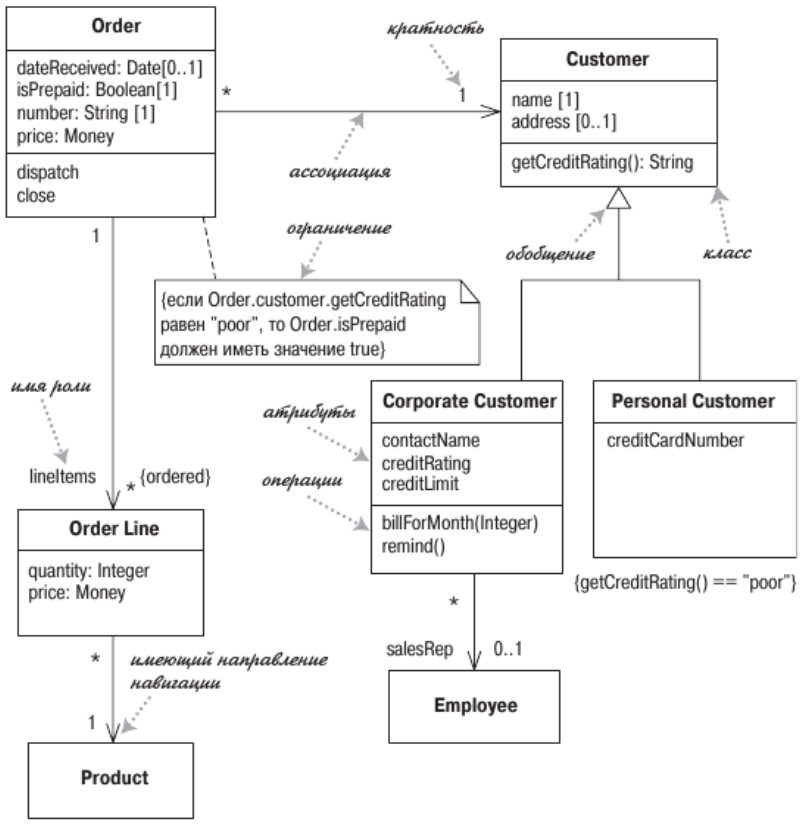
\includegraphics[height=0.8\textheight]{umlClassDiagram.png}
            \attribution{М. Фаулер. ``UML. Основы''}
        \end{center}
    \end{frame}

    \begin{frame}
        \frametitle{Частые ошибки}
        \begin{itemize}
            \item Если есть ассоциация, то не надо рисовать поле
            \item Не надо писать над стрелками их смысл
            \begin{itemize}
                \item Должны быть говорящие имена ролей (поля)
                \item Либо комментарии
            \end{itemize}
            \item Не путайте направления генерализаций
            \item Ромбик рисуется у <<хозяина>>
            \item Наследование от класса и реализация интерфейса --- разные вещи
            \item Не надо старательно выписывать каждое поле и метод
            \item Обращайте внимание на синтаксис параметров и возвращаемого значения
            \item Старайтесь использовать множественность вместо классов-контейнеров
        \end{itemize}
    \end{frame}

    \begin{frame}
        \frametitle{Диаграммы компонентов}
        \begin{center}
            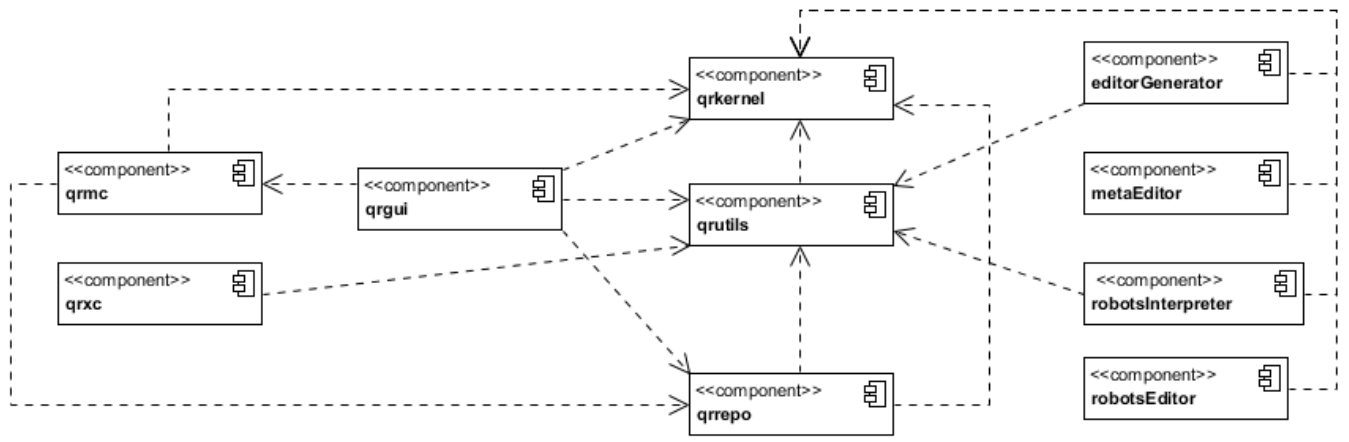
\includegraphics[width=0.95\textwidth]{componentDiagrams.png}
        \end{center}
    \end{frame}

    \begin{frame}
        \frametitle{Диаграмма развёртывания UML}
        \begin{columns}
            \begin{column}{0.5\textwidth}
                \begin{itemize}
                    \item Узлы --- реальные (или виртуальные) устройства
                    \item Связи --- каналы данных между узлами (не компонентами)
                    \item Связи подписываются протоколом
                \end{itemize}
            \end{column}
            \begin{column}{0.5\textwidth}
                \begin{center}
                    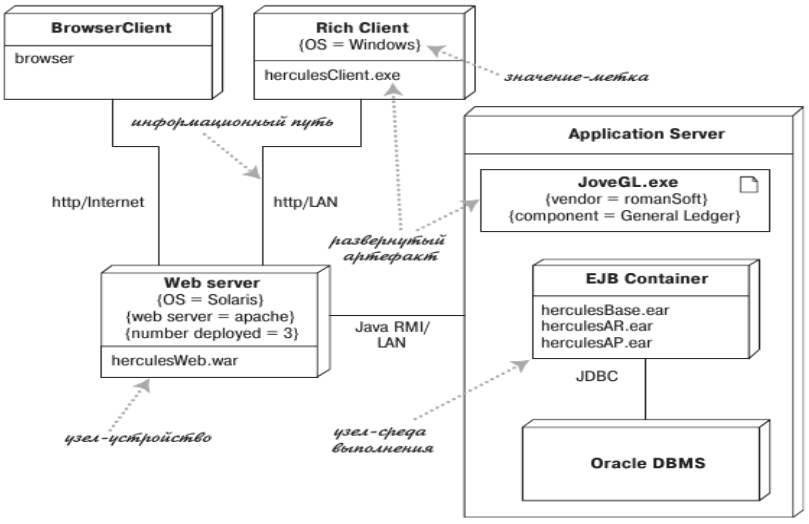
\includegraphics[width=\textwidth]{deploymentDiagram.png}
                    \attribution{М. Фаулер, UML. Основы}
                \end{center}
            \end{column}
        \end{columns}
    \end{frame}

    \begin{frame}
        \frametitle{Задачи на пару}
        \begin{itemize}
            \item Вспомнить запрос \url{https://goo.gl/MiyH8c}
            \item Задача 1: Построить \textit{модель данных} разрабатываемого приложения в виде диаграммы классов
            \item Задача 2: Нарисовать диаграмму компонентов разрабатываемого приложения
            \begin{itemize}
                \item То есть первое приближение архитектуры
            \end{itemize}
            \item Задача 3: Нарисовать диаграмму развёртывания разрабатываемого приложения
            \item Пользоваться одним из CASE-инструментов с лекции
            \begin{itemize}
                \item Расшарьте проект сразу, я буду комментировать по ходу
            \end{itemize}
            \item Отчуждаемый результат --- ссылка на проект с диаграммой в решение в MS Teams
            \begin{itemize}
                \item Не забудьте расшарить
            \end{itemize}
            \item В 16:50 встречаемся в общем чате и показываем пару решений
        \end{itemize}
    \end{frame}

\end{document}
